\section{Teori}
\subsection{Grundlæggende}
\begin{frame}{Occupancy Grid}
\begin{figure}[h] % Kørselsmiljø og et occupancy grid
\centering
	\begin{subfigure}[b]{.48\textwidth}
	\centering
	\includegraphics[width=\textwidth]{verden/oppefra_m_walle}
	\caption{Aktuelt Kørselsmiljø.}
	\label{map:world}
	\end{subfigure}
	\hfill
	\begin{subfigure}[b]{.48\textwidth}
	\centering
	\includegraphics[width=\textwidth]{verden/occupancy_grid_verden}
	\caption{Occupancy Grid.}
	\label{map:occupancy_grid}
	\end{subfigure}

\end{figure}
\end{frame}
\begin{frame}{Bayes Regel}
Opdatering af troen på en proposition ved ny evidens
\[
\begin{split}
P(h \mid e) = \frac{P(e \mid h) \times P(h)}{P(e)}
\end{split}
\]
\end{frame}

\begin{frame}{Log Odds}
\begin{figure}
\centering \includegraphics[scale=.2]{LogOdds}
\label{logoddsimg}
\end{figure}

%Log odds er en metode der kan benyttes for at undgå, at komponenterne i Bayes Regel enten bliver definitivt sande eller falske.
%
%Der kan derfor indføres en funktion, \textit{log odds ratio}, som mapper sandsynlighedsværdierne fra $[0;1]$ til $[-\infty;\infty]$.
%Oddset for tilstand $x$ er defineret som forholdet mellem sandsynlighederne for $x$ og $\lnot x$: 

\begin{tabular}{ p{0.5\linewidth} p{0.5\linewidth} }
$ l(x) = \log \frac{p(x)}{1 - p(x)} $ & 
$ bel_t(x) = 1 - \frac{1}{1 + exp\{l_x\}}\label{logodds:bel} $
\end{tabular}
\end{frame}

\subsection{Occupancy Grid}

\begin{frame}{Binært Bayes Filter}
Kan bruges når verdenens tilstand er statisk

\begin{algorithm}[H]
\textbf{BinaryBayesFilter($l_{t-1}, z_t$)} \\
\Indp $l_t = l_{t-1} + \log \frac{p(x \mid z_t)}{1-p(x \mid z_t)} - \log \frac{p(x)}{1-p(x)}$ \\
\Return{$l_t$}
\end{algorithm}
\end{frame}

\begin{frame}{Occupancy grid}
\begin{algorithm}[H]
OccupancyGridMapping(\{$l_{t-1,i}$\}, $x_t$, $z_t$):

\ForAll{cells $ m_i $}
{
\eIf{$ m_i $ is in the perceptual field of $ x_t $}
%then
{ $ l_{t,i} = l_{t-1,i} $ + \textbf{inverse\_sensor\_model} $( m_i, x_t, z_t ) - l_0$\\ }
%else
{ $ l_{t,i} = l_{t-1,i}  $\\ }
}
\Return {$ \{l_{t,i}\} $}
\end{algorithm}
\end{frame}

\begin{frame}{Occupancy grid}
\begin{algorithm}[H]
OccupancyGridMapping(\{$l_{t-1,i}$\}, $x_t$, $z_t$):

\ForAll{cells $ m_i $}
{
\eIf{$ x_i = x_r$ or $y_i = y_r$}
%then
{ $ l_{t,i} = l_{t-1,i} $ + \textbf{inverse\_sensor\_model} $( m_i, x_t, z_t ) - l_0$\\ }
%else
{ $ l_{t,i} = l_{t-1,i}  $\\ }
}
\Return {$ \{l_{t,i}\} $}
\end{algorithm}
\end{frame}

\subsection{Sensormodeller}
\begin{frame}{Simpel sensormodel}

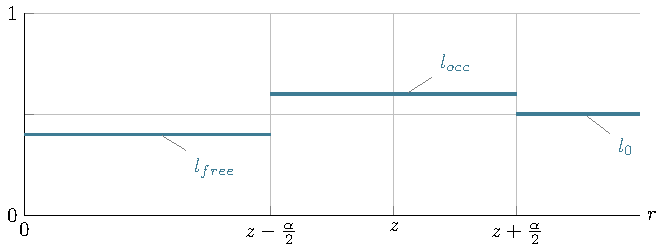
\includegraphics{simple_sensormodel.pdf}
\end{frame}

\begin{frame}{Gaussisk sensormodel}

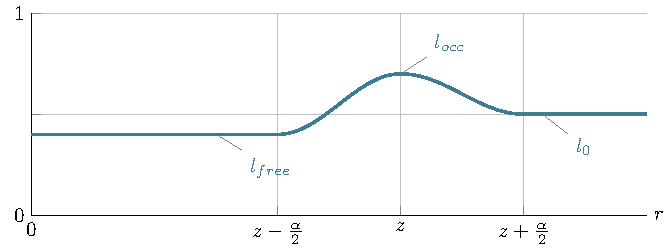
\includegraphics{gaussian_sensormodel.pdf}
\end{frame}

\begin{frame}{Sammenligning af sensormodeller}
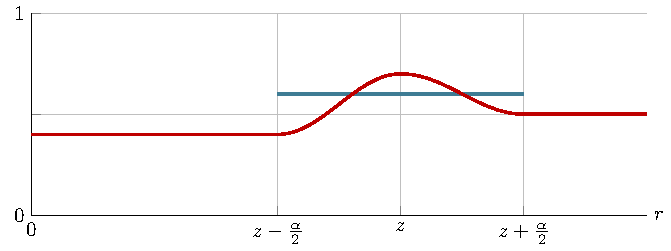
\includegraphics{combined_sensormodel}
\end{frame}

